\chapter{Band Bendings}
\label{chap:bandbend}

At this point we begin to have a fairly clear picture of the TiO$_2$-based memristor: the oxygen-deficient phases that arise inside the active layer of the device are responsible for a new ingredient, the intermediate band, which in turn can be charged and de-charged and moreover, $n$-dope the surrounding TiO$_2$ structure. This is enough evidence to consider an electronic model for memristors. In fact, a very similar model has already been proposed for gold impurities inside a SiO$_2$ thin film by Simmons \cite{Simmons1967} long before the discussion about the memristor became popular. Experimental reports at nearly the same time also claim that the transport phenomena could be related to space charge conduction on oxide thin films \cite{Argall1968,Chopra1965}.

However, the so-called \textit{voltage-time dilemma} for purely electronic models claim that the average lifetime of the different charge states---and consequent different resistance states---would be much shorted than the retention times reported \cite{Schroeder2010}. For this reason, many models based on the ionic drift-diffusion of impurities inside the memristor were proposed and became popular among experimentalists. Ielmini \textit{et al.} proposed a \textit{field- and/or temperature-enhanced acceleration} model for ions, which could form and dissolve a conductive channel inside a HfO$_2$ memristor \cite{Ielmini2011,Ielmini2012}. %Curiously, the timescale obtained by direct or indirect measurements for these processes is of the order of seconds or minutes \cite{Yang2014,Kudo2014}, while the reported switching times can reach nanoseconds or even picoseconds \cite{Pan2014}.

The key point is that in most of the claims supporting the ionic drift models and criticizing the electronic models, the profile of the potential energy inside the active region of memristors is assumed to be of a certain shape. For the voltage-time dilemma, typical metal-insulator \textit{band bendings} are assumed as solutions to Poisson equation and the resulting barriers are approximated by triangles or trapezoids \cite{Schroeder2010}, while for the accelerated ionic motion models the potential is assumed to be a straight line (constant electric field across the active region) \cite{Ielmini2011,Ielmini2012}. Unfortunately, no explicit solution of the Poisson equation is presented in the literature. The role of the electronic processes in the switching is readily discarded, but there is no reason, in principle, to consider that either the electronic models or the ionic models should be considered as the only driving force of the mechanism. The assessment of the importance of the electronic contribution is the subject of this chapter, where the solution of the Poisson equation for fixed ions is presented.

\section{Solving the Poisson equation}
\label{sec:poisson}

As a first approximation, the memristor can be modeled as a 1D device\footnote{Owing to periodic boundary conditions in the transverse ($x$ and $y$) coordinates, the potential is constant in these directions.}, thus, the total energy of the system can be written as a functional of the electrostatic potential $\phi$,
\begin{equation}
	F[\phi(z)] = \int_a^b \mathrm{d}z \left[ \frac{1}{2}\left( \frac{\mathrm{d}\phi}{\mathrm{d}z}\right)^2+\frac{\phi \rho}{\epsilon \epsilon_0}\right],
	\label{eq:poisson}
\end{equation}
where $z$ is the direction perpendicular to the metal/semiconductor interface, $\rho$ is the charge density along this direction, and $\epsilon$ and $\epsilon_0$ are the relative and vacuum permittivities respectively. This expression comprises the energy density of the electric field ($|\vec{E}|^2=(\mathrm{d}\phi/\mathrm{d}z)^2$) and the same quantity due to the interaction between the charge density and the potential. The function $\phi$ that minimizes \ref{eq:poisson} is the solution to the Poisson equation, \textit{i. e.} the electrostatic potential. The Euler-Lagrange equation for this functional is
\begin{equation}
	\frac{\mathrm{d}^2 \phi}{\mathrm{d}z^2}=\frac{\rho}{\epsilon \epsilon_0} + \frac{\phi}{\epsilon \epsilon_0}\frac{\partial \rho}{\partial \phi}.
	\label{eq:euller-lagrange}
\end{equation}

Owing to the fact that the charges are not fixed inside the active layer of the memristor, $\rho$ is a functional of $\phi$, \textit{i.e.}, $\rho = \rho[\phi(z),z]$, and its expression is given by
\begin{equation}
	\rho = -n_e + n_h + N_D(q_D - n_D)
	\label{eq:charge-density}
\end{equation}
where $N_D$, and $n_D$ are respectively the concentration, and the charge state of defects inside the active region, $q_D$ the number of electrons trapped in these defects, while $n_e$ and $n_h$ are the concentrations of electrons in the CB and holes in the VB respectively, which are given by
\begin{equation}
	n_e = \int_{\phi}^{+\infty} \frac{g_c(\varepsilon)\mathrm{d}\varepsilon}{e^{\nicefrac{\varepsilon}{kT}}+1}, \qquad
	n_h = \int_{-\infty}^{\phi-E_g} \frac{g_v(\varepsilon)\mathrm{d}\varepsilon}{e^{\nicefrac{-\varepsilon}{kT}}+1},
	\label{eq:e-h-dens}
\end{equation}
where $k$ is Boltzmann's constant, $T$ is the temperature, $\varepsilon$ is the energy, and $g_c$ and $g_v$ are the density of states for the electrons in CB and holes in VB respectively, given by
\begin{equation}
	g_c(\varepsilon) = \frac{m_c^{*\nicefrac{3}{2}}}{\hbar^3 \pi^2}\sqrt{2(\varepsilon-\phi)}, \qquad
	g_v(\varepsilon) = \frac{m_v^{*\nicefrac{3}{2}}}{\hbar^3 \pi^2}\sqrt{2(\phi-E_g-\varepsilon)},
\end{equation}
where $m_c^*$ and $m_v^*$ are the effective masses of electrons and holes respectively, $\hbar = \nicefrac{h}{2\pi}$ is Planck's constant and $E_g$ is the bandgap energy. Finally, the occupation of the defect levels is given by a Boltzmann distribution,
\begin{equation}
	n_D = \frac{\sum_j N_j e^{\nicefrac{-\varepsilon_j}{kT}}}{\sum_j e^{\nicefrac{-\varepsilon_j}{kT}}}.
\end{equation}
where $\varepsilon_j$ and $N_j$ are the energy and number of electrons in state $j$ within the bandgap. Equation \ref{eq:euller-lagrange} can be discretized by rewriting the second derivative as
\begin{equation}
	\frac{\mathrm{d}^2 \phi}{\mathrm{d}z^2} \approx \frac{\phi_{i-1}-2\phi_i+\phi_{i+1}}{h^2}, \qquad 1 \leq i \leq N,
\end{equation}
where $h = \nicefrac{(b-a)}{N}$ is the finite element in a real-space grid, $\phi_j = \phi(z_j)$ is the electrostatic potential in the $j$-th grid point, and imposing Dirichlet boundary conditions $\phi_0 = \phi(a) = \phi_a$, and $\phi_{N+1} = \phi(b) = \phi_b$, which correspond to the Schottky barriers at the insulator/metal interfaces, the final result can be written in matrix form,
\begin{equation}
\tiny
	\left[ 
		\begin{array}{cccccc}
 			-\frac{2}{h^2}-\frac{\partial_{\phi} \rho_1}{\epsilon \epsilon_0} & \frac{1}{h^2} & 0 & 0 & \cdots & 0 \\
 			\frac{1}{h^2} & -\frac{2}{h^2}-\frac{\partial_{\phi} \rho_2}{\epsilon \epsilon_0} & \frac{1}{h^2} & 0 & \cdots & 0 \\
 			\vdots & \vdots &  & &  & \vdots \\
 			0 & 0 & \cdots & \frac{1}{h^2} & -\frac{2}{h^2}-\frac{\partial_{\phi} \rho_{N-1}}{\epsilon \epsilon_0} & \frac{1}{h^2} \\
 			0 & 0 & \cdots & 0 & \frac{1}{h^2} & -\frac{2}{h^2}-\frac{\partial_{\phi} \rho_N}{\epsilon \epsilon_0}
		\end{array} 
	\right] 
	\left[
		\begin{array}{c} 
			\phi_1 \\ 
			\phi_2 \\ 
			\vdots \\ 
			\phi_{N-1} \\
			\phi_N 
		\end{array} 
	\right] 
	= 
	\left[
		\begin{array}{c}
			\frac{\rho_1}{\epsilon \epsilon_0} - \phi_a \\ 
			\frac{\rho_2}{\epsilon \epsilon_0} \\ 
			\vdots \\ 
			\frac{\rho_{N-1}}{\epsilon \epsilon_0} \\
			\frac{\rho_N}{\epsilon \epsilon_0} - \phi_b
		\end{array}
	\right]
	\normalsize
	\label{eq:matrix-euller-lagrange}
\end{equation}
where the derivatives $\partial_{\phi} \rho_i =\nicefrac{\partial \rho_i}{\partial \phi}$ are obtained numerically by finite differences. According to equations \ref{eq:charge-density} and \ref{eq:e-h-dens}, the charge density is a functional of the potential, $\rho = \rho[z,\phi(z)]$, thus, we start from a parabolic \textit{ansatz} for $\phi$ and evaluate $\rho$ by numerical integration.
\begin{center}
  \begin{figure}[h!]
    \begin{center}
      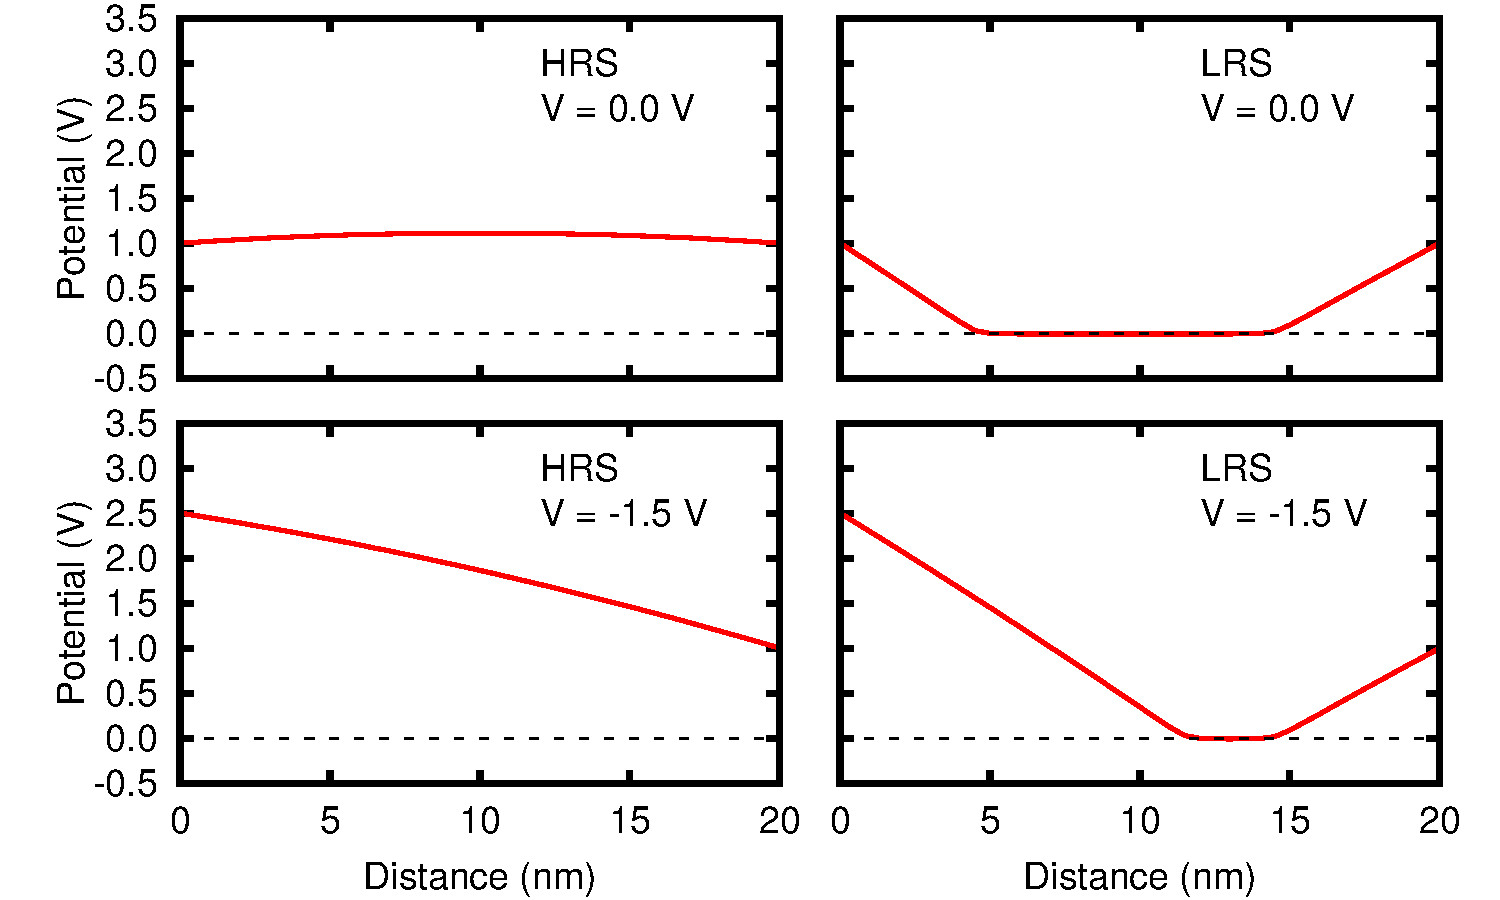
\includegraphics[width=0.8\textwidth]{img/switch-2x2.jpg}    
      \caption{Multiple solutions of the Poisson equation for a 20 nm wide memristor. The curves are the potential barrier for charges to flow through the device. The dashed horizontal line depicts the Fermi Level. The HRS is featured in the left column while the LRS for the corresponding voltage is featured in the right column.} 
      \label{fig:multiple-poisson} 
    \end{center}
  \end{figure}
\end{center}

Using these results in equation \ref{eq:matrix-euller-lagrange} we solve the system numerically \footnote{By use of a Lapack routine \cite{lapack}} and obtain the first iteration, subsequently calculating the potential in every point of the real-space grid $\phi_j$. This result allows the calculation of a new charge density by integration of equations \ref{eq:e-h-dens} and substitution into \ref{eq:charge-density}. The \textit{self-consistent solution} to this set of equations is obtained by repeating this process until the Dirichlet energy (equation \ref{eq:poisson}) is converged. The resulting $\phi$ are the potential barriers for electrons to flow through the active region, which in this case presents multiple stable solutions, \textit{i. e.} there are two solutions, one is the High Resistance State (HRS) while the other is the Low Resistance State (LRS), for a given potential, as shown in figure \ref{fig:multiple-poisson}. 
\begin{center}
  \begin{figure}[h!]
    \begin{center}
      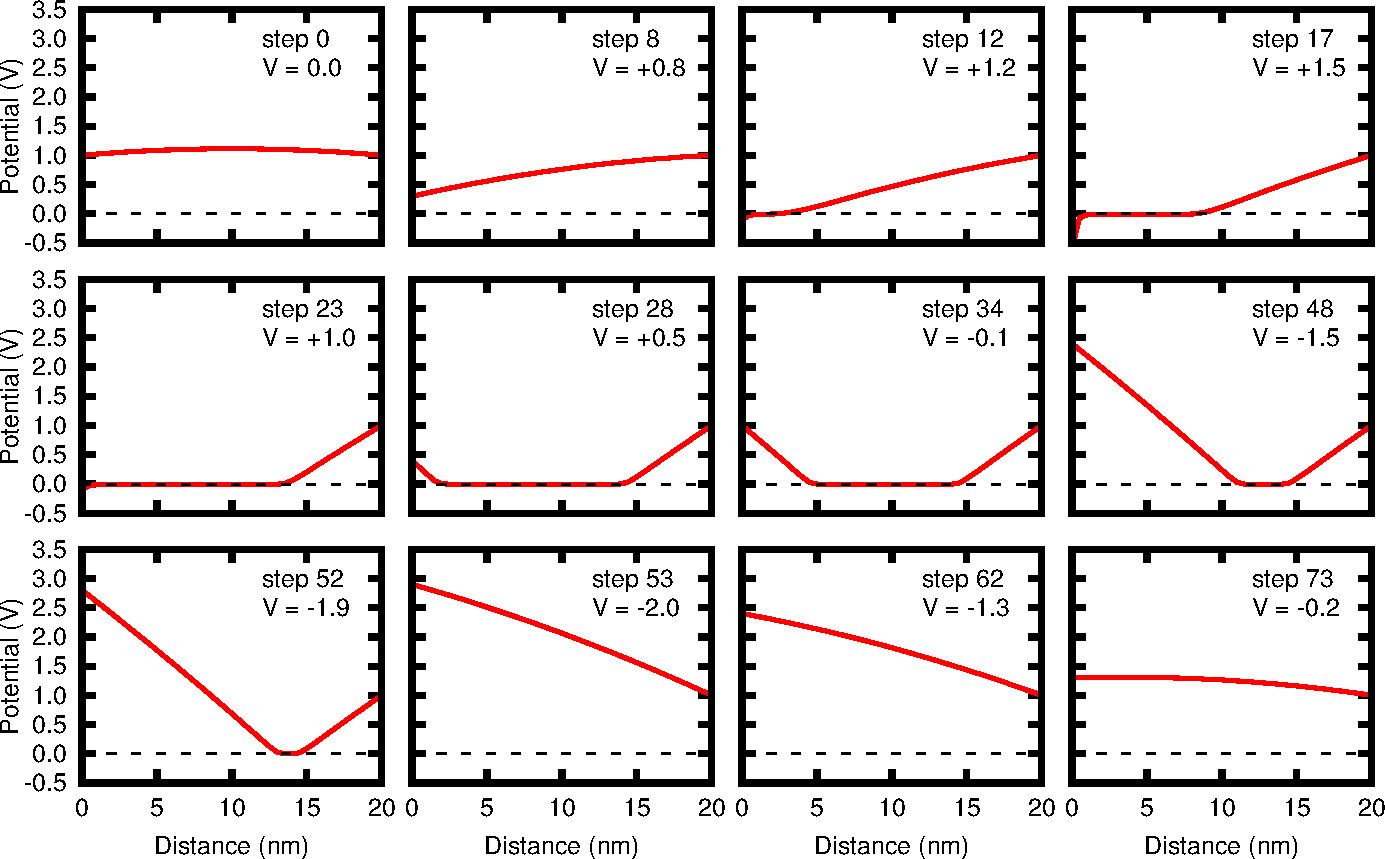
\includegraphics[width=0.9\textwidth]{img/switch-4x3.jpg}    
      \caption{Snapshots of the resulting potential energy barriers for a 20 nm wide memristor. The dashed horizontal line depicts the Fermi Level. Each step is an increase or decrease of 0.1 V, which is basically the height of the Schottky barrier at the electrode at the origin.} 
      \label{fig:potentials} 
    \end{center}
  \end{figure}
\end{center}

More results obtained from the code implemented by Dr. Raebiger are presented in figure \ref{fig:potentials}. For each run the dielectric Schottky barrier at the right electrode is kept fixed at 1 V ($\phi_b = 1$) while the left electrode barrier is varied according to the voltage. The first switch takes place at step 12, when $\phi$ touches the Fermi level and the device goes from HRS to LRS. From step 17 to step 52, the left barrier $\phi_a$ is raised\footnote{Our convention is that the voltage $V = 0$ if the Schottky barrier $\phi_a = 1$ V. When the voltage is raised the barrier is lowered and vice-versa.} and in step 53 $\phi$ \textit{detaches} from the Fermi level abruptly: this is the switching from LRS to HRS.
\begin{center}
  \begin{figure}[h!]
    \begin{center}
      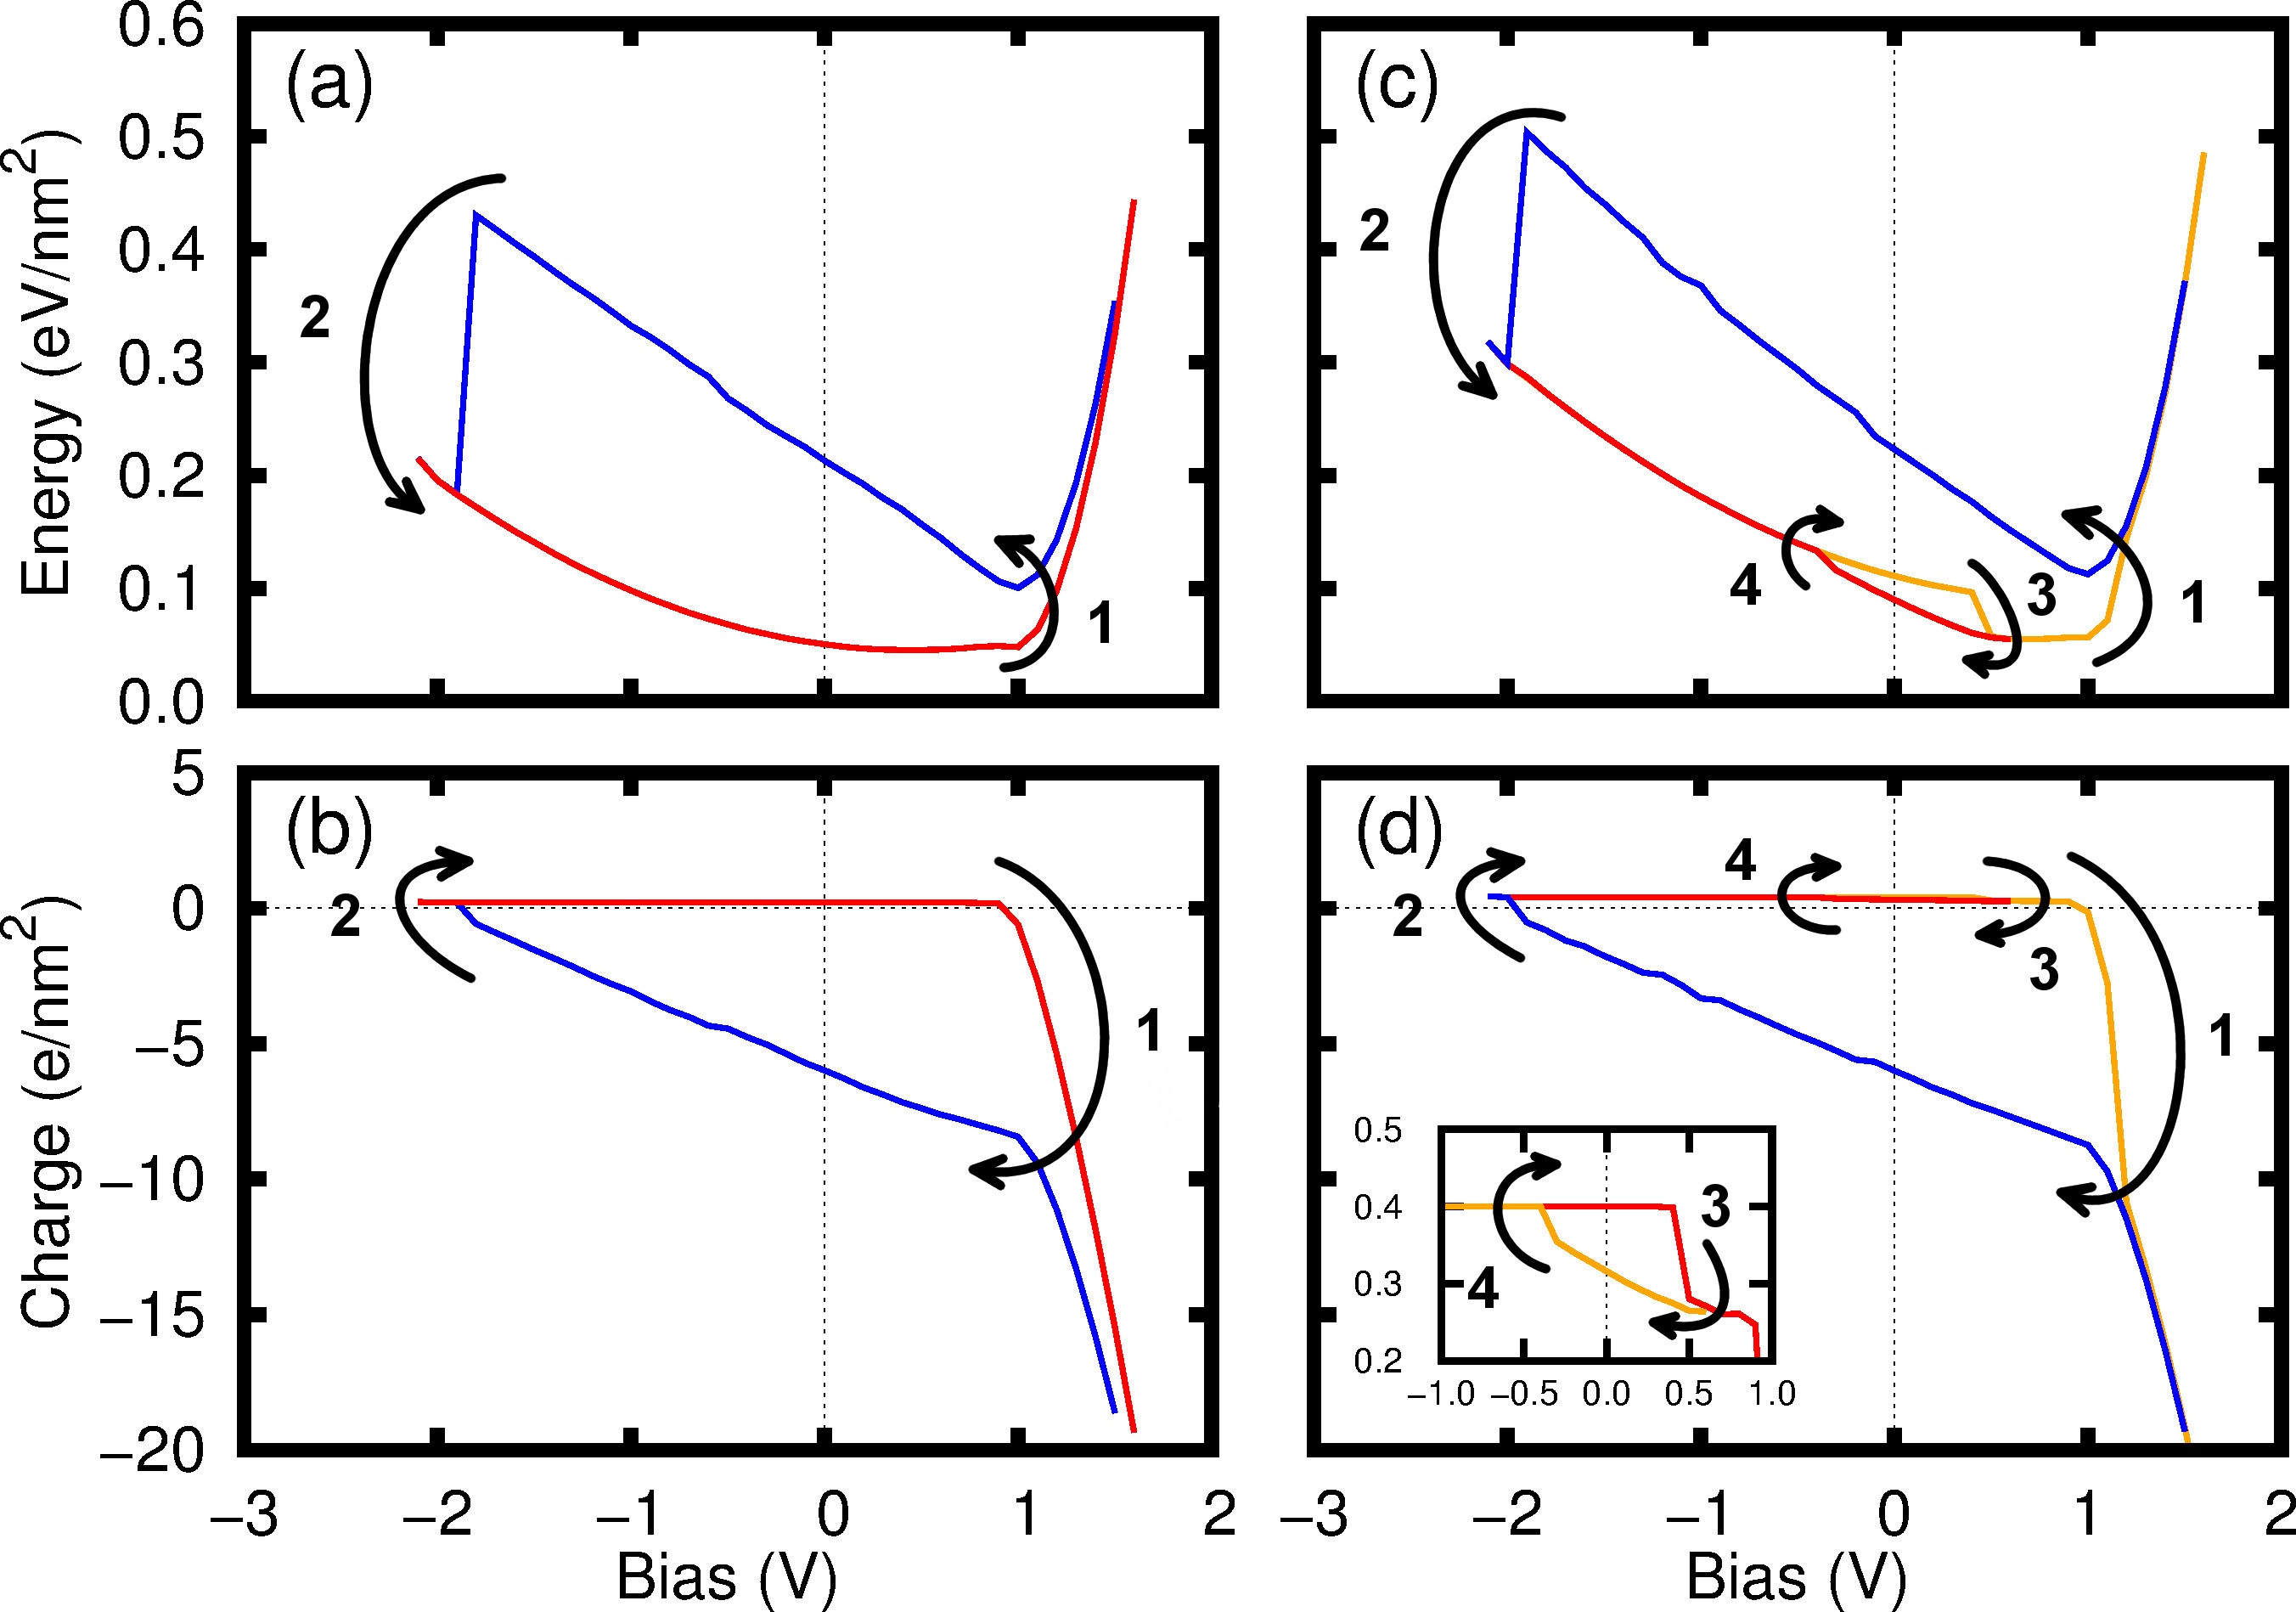
\includegraphics[width=0.8\textwidth]{img/charge-energy.jpg}    
      \caption{Total energy $F$ (given by equation \ref{eq:poisson}) for defect scenarios: (a) i) a homogeneous concentration of $5 \cdot 10^{-3} \, \text{nm}^{-3}$ of $V_{\text{O}}$, and (c) ii) homogeneous concentration of $5 \cdot 10^{-3} \, \text{nm}^{-3}$ of Ti$_i$ together with $2.5 \cdot 10^{-3} \, \text{nm}^{-3}$ of $V_{\text{O}}$. Total charge $Q$ for scenarios: (b) i), and (d) ii). Switch between LRS and HRS is shown by arrows labeled 1 and 2, while arrows 3 and 4 depict the switching to and from the IRS. The inset in (d) shows the hysteresis loop for the switching between HRS and IRS.} 
      \label{fig:charge-energy} 
    \end{center}
  \end{figure}
\end{center}

The total charge $Q$, obtained by integrating the resulting $\rho$ on the real-space grid, is shown to be distinct for the two solutions, as well as the Dirichlet (or total) energy $F$ of the system, given by equation \ref{eq:poisson}, as presented in figure \ref{fig:charge-energy} for two homogeneous defect concentration scenarios: i) $5 \cdot 10^{-3} \, \text{nm}^{-3}$ of oxygen vacancies ($V_{\text{O}}$), and ii) $5 \cdot 10^{-3} \, \text{nm}^{-3}$ of titanium interstitials (Ti$_i$) with $2.5 \cdot 10^{-3} \, \text{nm}^{-3}$ of $V_{\text{O}}$. An intermediate resistance state (IRS) is detected in scenario ii), due to the multiple defect states present within the bandgap. In these graphs one can see two [defect scenario i)] or three [defect scenario ii)] distinct values of energy or charge for each value of the applied voltage. By raising or lowering the voltage the distinct curves overlap and the switching occurs. Arrows 1 and 2 are respectively the reset and set processes in defect scenario i) [figure \ref{fig:charge-energy} (a) and (b)], while arrows 1 and 2 play the same role for defect scenario ii) with an additional hysteresis loop from HRS to IRS and back described by arrows 3 and 4 [figure \ref{fig:charge-energy} (c) and (d)]. While for HRS and IRS the total charge is slightly positive for the most part of the switching cycle, the LRS shows an accumulation of negative charge. This is consistent with a scenario where the HRS and IRS present fully or partially ionized defect levels and poor conduction, while the LRS is such that band conduction is possible owing to the presence of electrons in the CB of the material.
\begin{center}
  \begin{figure}[h!]
    \begin{center}
      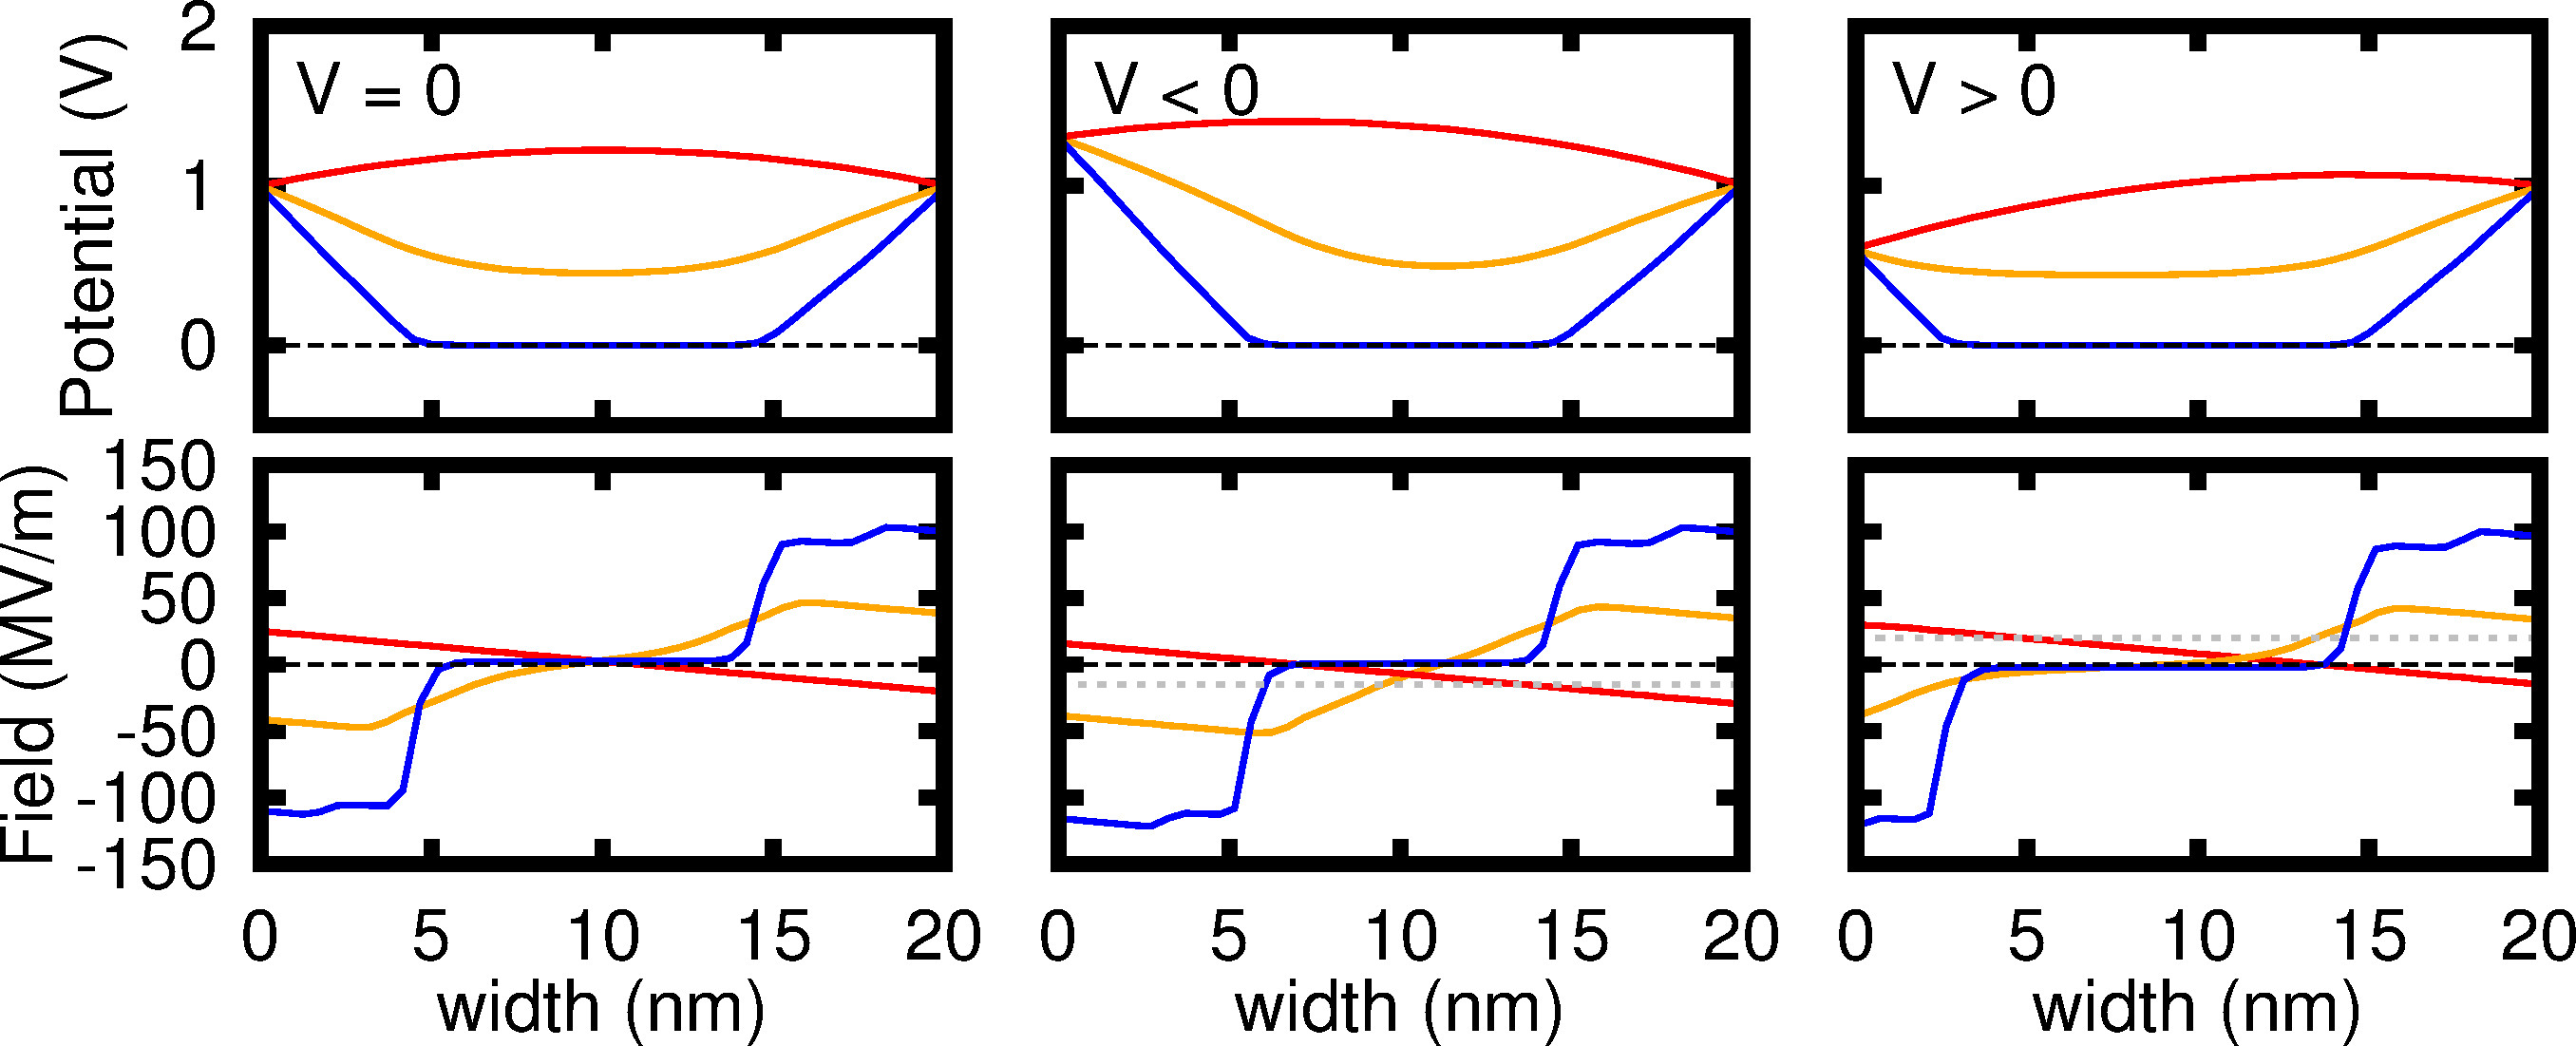
\includegraphics[width=0.8\textwidth]{img/field.jpg}    
      \caption{Potentials $\phi$ and corresponding electric fields $E$ for HRS (red), IRS (orange), and LRS (blue) in defect scenario ii) and different applied voltages. The gray dashed line depicts the constant electric field $E_0 = V/L$ for comparison.} 
      \label{fig:field-pot} 
    \end{center}
  \end{figure}
\end{center}

The electric field $E = \partial \phi / \partial z$\footnote{Notice that the signal convention is not the usual here due to the fact that we are interested in the barriers for electrons.} and corresponding potential $\phi$ for defect scenario ii) are shown in figure \ref{fig:field-pot}, where one can see huge electric fields close to the electrodes. These fields are responsible for expelling electrons from the active media while the system is in HRS and doing the opposite in the LRS and IRS. See for example figure \ref{fig:field-pot} (a) where $E > 0$ close to the left electrode and $E < 0$ close to the opposing electrode for the HRS state and vice-versa for LRS and IRS. In this situation, the HRS state responds to an insertion of electrons by expelling them, and the LRS does the opposite: these are stationary solutions. Of course, the large values of the electric field close to the electrodes might lead to ionic migration, or even to the breakdown of the material. Such extreme situation might be avoided by a rearrangement of the defects in these interfacial layers, as it is detected by experiments \cite{Kwon2010,Szot2011,HwanKim2011}.
\begin{center}
  \begin{figure}[h!]
    \begin{center}
      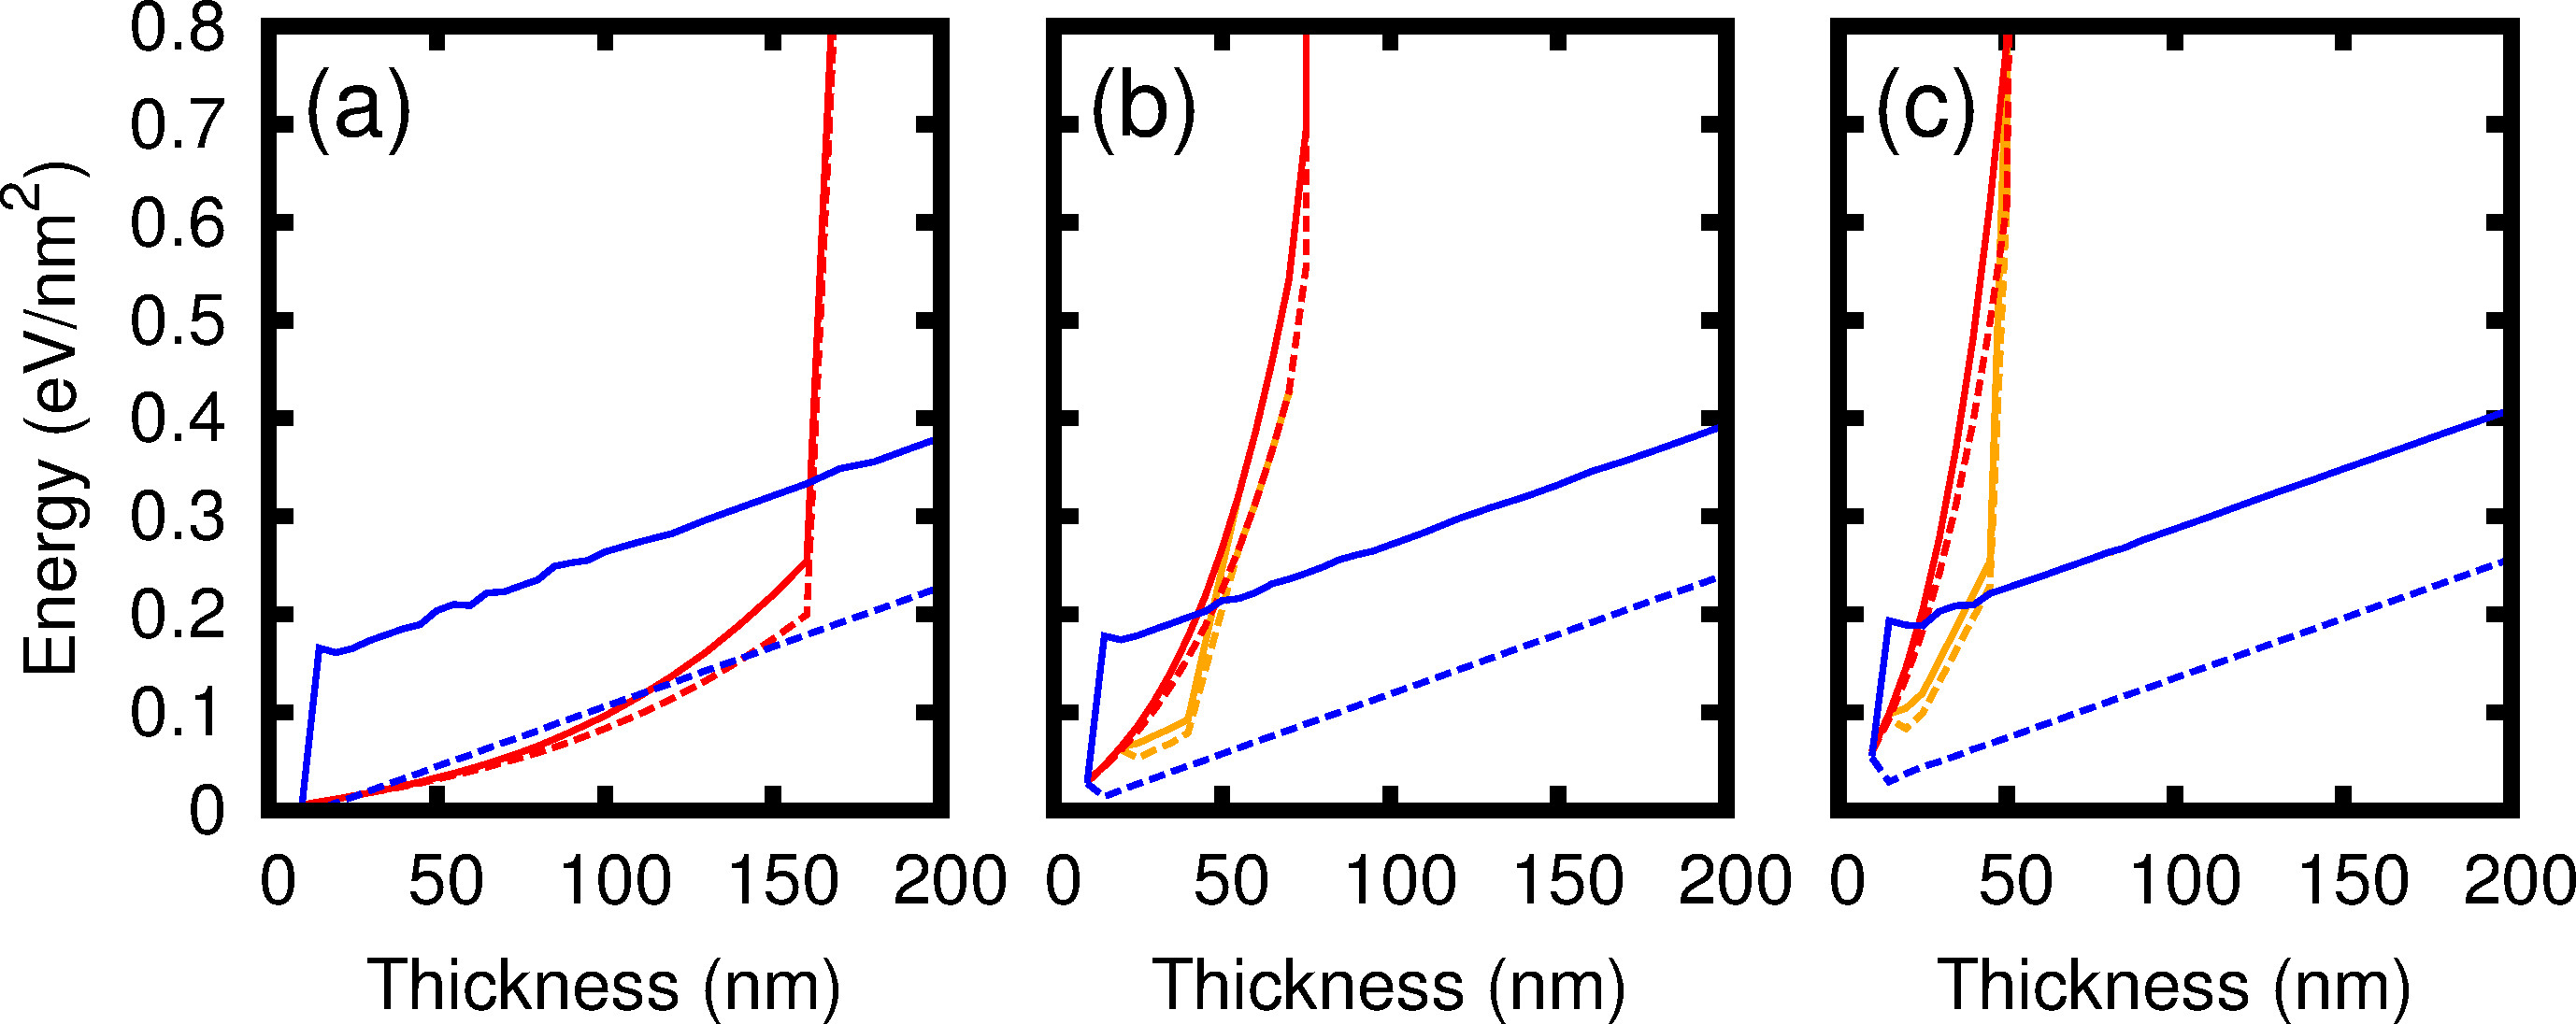
\includegraphics[width=0.8\textwidth]{img/energy-width.jpg}    
      \caption{Total energy $F$ (solid lines) and its contribution due to the interaction between charge density and potential $F_{\rho} = \int_a^b \mathrm{d}z \left(\nicefrac{\rho \phi}{\epsilon \epsilon_0}\right)$ (dashed lines) as a function of device width $L$. HRS, IRS, and LRS are the red, orange, and blue curves respectively. Defect concentrations are: (a) $1.0 \cdot 10^{-3} \, \text{nm}^{-3}$, (b) $5.0 \cdot 10^{-3} \, \text{nm}^{-3}$, and (c) $1.0 \cdot 10^{-2} \, \text{nm}^{-3}$ of homogeneously distributed $V_{\text{O}}$ and half these values of Ti$_i$.} 
      \label{fig:fxl} 
    \end{center}
  \end{figure}
\end{center}

Finally, the sensitivity to device parameters is assessed for our memristor model. By controlling the width of the device ($L = b - a$) and the concentration of defects ($N_D$), as well as the defect state charge $q_{D,0}$ and energy $E_D$ with respect to CBM, different profiles are obtained. Plots of the total energy $F$ and $F_{\rho} = \int_a^b \mathrm{d}z \left(\nicefrac{\rho \phi}{\epsilon \epsilon_0}\right)$, the contribution to $F$ arising from the interaction between the charge density $\rho$ and the potential $\phi$ with respect to the device width $L$ are shown in Figure \ref{fig:fxl} for various defect concentrations. For higher concentrations, both $F$ and $F_{\rho}$ diverged quickly as the thickness increases, owing to the fact that larger charges are stored inside the device in this case, leading to strong electrostatic repulsion. This shows that the interplay between defect concentration and the thickness of the device might be responsible for the memristive property to arise at the nanoscale. Large defect concentrations, as provided by the Magnéli phases fit in this model. %All results shown here are once more presented in our preprint \cite{Raebiger2014} (appendix \ref{sec:app-sub}).

\section{Electronic Transport}
\label{sec:transport}

The simplest model for the electronic transport across the device consists of scattering and/or tunneling of electrons through a potential energy barrier. Within our first approximation, electrons are regarded as free waves incident, reflected and transmitted across a 1D barrier. The corresponding wavefunctions in the neighboring regions to the active region are
\begin{equation}
	\psi_L(z) = e^{ik_Lz}+re^{-ik_Lz}, \qquad
	\psi_R(z) = te^{ik_Rz},
	\label{eq:wavefunct}
\end{equation}
where $k_{L/R}=\sqrt{\nicefrac{2m}{\hbar^2}(\varepsilon-U_{L/R})}$ are the 1D wave vectors of the electrons in the left and right electrodes respectively, and $\varepsilon$ is the total energy of the electron. 

\begin{center}
  \begin{figure}[h!]
    \begin{center}
      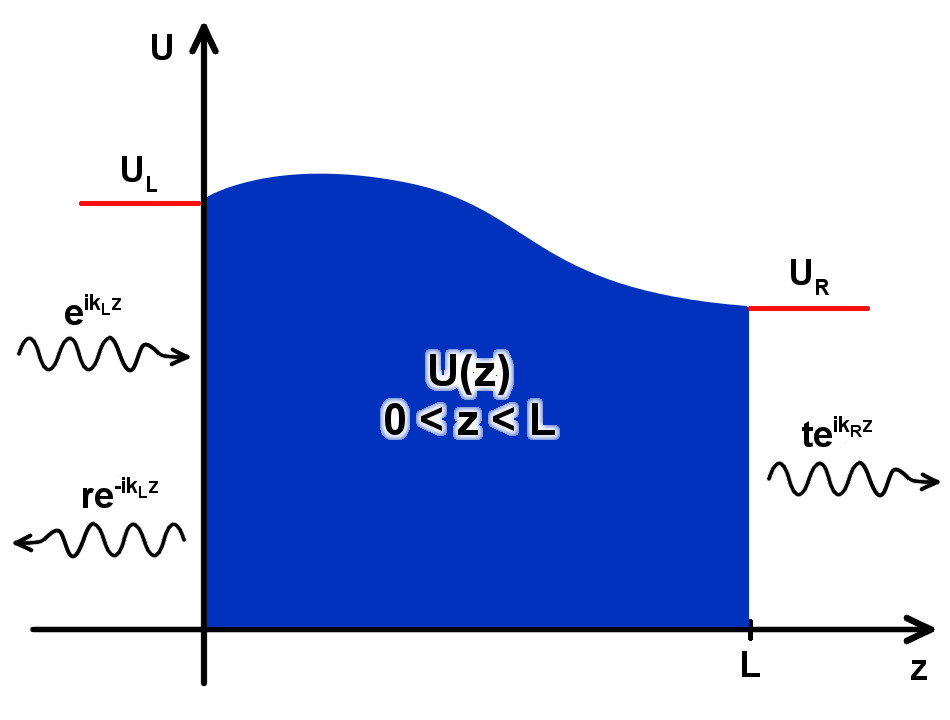
\includegraphics[width=0.6\textwidth]{img/transm-01.jpg}    
      \caption{Diagram of the electron tunneling process across a 1D memristor of width $L$. The potential $U(z)$ is obtained from the Poisson solver while the right electrode potential $U_R$ is kept fixed and the left electrode potential $U_L$ is varied.} 
      \label{fig:transm-01} 
    \end{center}
  \end{figure}
\end{center}

The diagram in figure \ref{fig:transm-01} depicts this situation. According to what was done in the solution of the Poisson equation, the potential in the right electrode is kept fixed for all calculations ($U_R = 1.0$ V) while the potential in the opposite electrode ($U_L$) is changed according to the voltage to which the device is subject. 

The wavefunction in the scattering region is the solution of the 1D single-particle time-independent Schr\"odinger equation
\begin{equation}
	-\frac{\hbar^2}{2m}\frac{\mathrm{d}^2}{\mathrm{d}z^2}\psi(z)+U(z)\psi(z)=\varepsilon \psi(z),
	\label{eq:schrodinger}
\end{equation}
which can be in turn discretized in the same way as it was done in the previous section, 
\begin{equation}
	\frac{\mathrm{d}\psi}{\mathrm{d}z}\approx \frac{\psi_i-\psi_{i-1}}{h}, \qquad 1 \leq i \leq N-1, 
\end{equation}
resulting in a finite-differences equation \cite{NR,King},
\begin{equation}
	\frac{1}{h^2}\psi_{j-1}+\left[ \frac{2m}{\hbar^2} (\varepsilon-U_j) - \frac{2}{h^2}\right] \psi_j + \frac{1}{h^2}\psi_{j+1}=0, \qquad 1 \leq j \leq N - 1,
	\label{eq:finite-diff-schrodinger}
\end{equation}
where $h = \nicefrac{L}{N}$ is one segment of the $N$-positions real-space grid, and $\psi_j = \psi(z_j)$ is the solution to the Schr\"odinger equation for a constant potential $U_j = U(z_j)$ in this segment. Imposing the continuity of the wavefunction at the metal/insulator interfaces $\psi_0=\psi_L(z_0)$, and $\psi_N=\psi_R(z_N)$, as well as for the derivatives $\psi_0'=\psi_L'(z_0)$, and $\psi_N'=\psi_R'(z_N)$, and eliminating $r$ and $t$ from these equations, it is possible to write equation \ref{eq:finite-diff-schrodinger} in matrix form
\begin{equation}
	%\begin{array}{cccc}
	\tiny
		\left[\begin{array}{cccccc}
			-\frac{1}{h}+ik_L & \frac{1}{h} & 0 & \dots & 0 & 0 \\
			\frac{1}{h^2} & k_1^2-\frac{2}{h^2} & \frac{1}{h^2} & \dots & 0 & 0 \\
			\vdots & \vdots & & \ddots & \vdots & \vdots \\
			0 & 0 & \dots & \frac{1}{h^2} & k_{N-1}^2-\frac{2}{h^2} & \frac{1}{h^2} \\
			0 & 0 & \dots & 0 & -\frac{1}{h} & \frac{1}{h}-ik_R
		\end{array}\right]
		\left[\begin{array}{c}
			\psi_0 \\ \psi_1 \\ \vdots \\ \psi_{N-1} \\ \psi_N
		\end{array}\right]
		=
		\left[\begin{array}{c}
			2ik_Le^{ik_Lz_0} \\ 0 \\ \vdots \\ 0 \\ 0
		\end{array}\right]
		\normalsize
		\label{eq:schroedinger-discrete-matrix}
	%\end{array}
\end{equation}
where $k_j^2 = \nicefrac{2m^*}{\hbar^2}(\varepsilon-U_j), 1 \leq j \leq N-1$. This equation is then solved numerically by a Fortran 90 code. The parameters used were $z_0 = 0$, $z_N = L = 20$ nm, the effective mass for electrons in TiO$_2$, $m^* = 0.8m_e$ (from DFT bandstructure calculations) while the values of $\varepsilon$ and $U_L$ were varied. Knowing the value of $\psi$ at the interfaces, it is straightforward to determine $r$ and $t$ from the equations used to impose the continuity of the wavefunction at these regions, $r = \psi_0-1$, $t=\psi_Ne^{-ik_RL}$. Thus, the probability of reflection $R$ and transmission $T$ is obtained by \cite{Cohen-Tannoudji}
\begin{equation}
T(U_{L/R},\varepsilon) = \left|\frac{k_R}{k_L}\right|^2|t|^2, \qquad
R(U_{L/R},\varepsilon) = |r|^2.
\end{equation}

At this point, the current is obtained from Landauer's model for the electronic transport at the nanoscale \cite{Datta}
 \begin{equation}
	I(U_L,U_R) = \frac{2e}{h} \int_{-\infty}^{+\infty}T(\varepsilon,U_{L/R}) \left[f(\varepsilon,U_L,T)-f(\varepsilon,U_R,T)\right] \mathrm{d}\varepsilon
\end{equation}
where $\nicefrac{2e}{h}$ is the quantum of conductance and $f_{L/R}$ are the Fermi-Dirac distributions at the electrodes. The temperature where the calculations took place was $T= 300$ K. The resulting $i \times V$ curve is presented in figure \ref{fig:ixvtheo-01} and it is compared with an experimental curve \cite{Pan2014}. The order of magnitude of the current for both high resistance (HR) and low resistance (LR) is very small in comparison with the experimental curve. A region of negative differential resistance is present for the LRS beyond 0.5 V which can be interpreted as a decrease in occupation in the CB (see Figure \ref{fig:potentials}, steps 17-52). Thus, it is an evidence of other transport mechanisms being responsible for the electronic current in the memristors.
\begin{center}
  \begin{figure}[h!]
    \begin{center}
      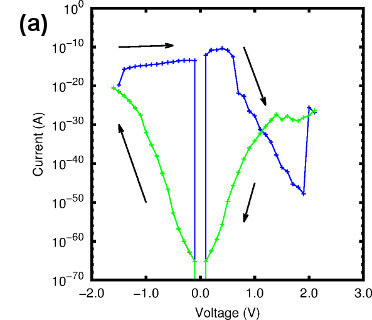
\includegraphics[height=5cm]{img/ixv-tunnel.jpg}    
      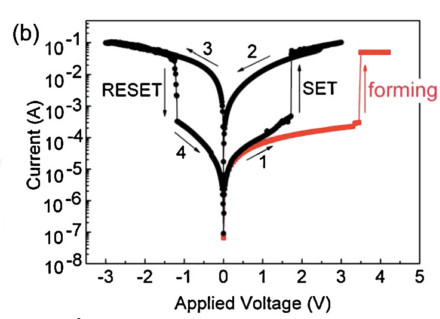
\includegraphics[height=5cm]{img/pan.jpg}    
      \caption{(a) theoretical and (b) experimental $i \times V$ curves of memristors \cite{Yang2009}. In (a) the blue curve is the LRS while the green one is the HRS.} 
      \label{fig:ixvtheo-01} 
    \end{center}
  \end{figure}
\end{center}

The role of the defect levels was not taken into account for the the transmission. A step in this direction is to consider a defect band inside the bandgap at $E_{CBM}-E_d$, as depicted in figure \ref{fig:ixvtheo-02} (a). In this case, the electrons are allowed to flow through this band in the same way they were considered to cross the CB. In practice, the CB is lowered by $E_d \approx 0.5$ eV in the region where it is higher than this value and considered zero everywhere else. This change led to a much more reasonable theoretical $i \times V$ curve, shown in figure \ref{fig:ixvtheo-02} (b). However, there is still an issue with respect to negative differential resistivity in the region $V > 0.5$ V for both the low and high resistivity curves, being the effect more pronounced for the first case. 
\begin{center}
  \begin{figure}[h!]
    \begin{center}
      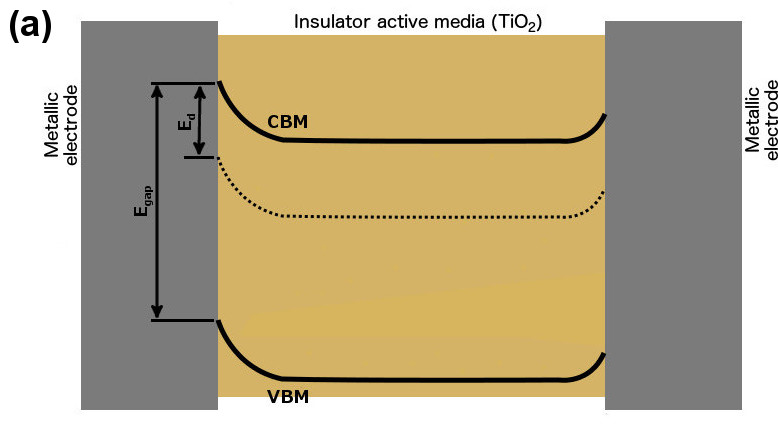
\includegraphics[height=4.5cm]{img/defect-band.jpg} 
      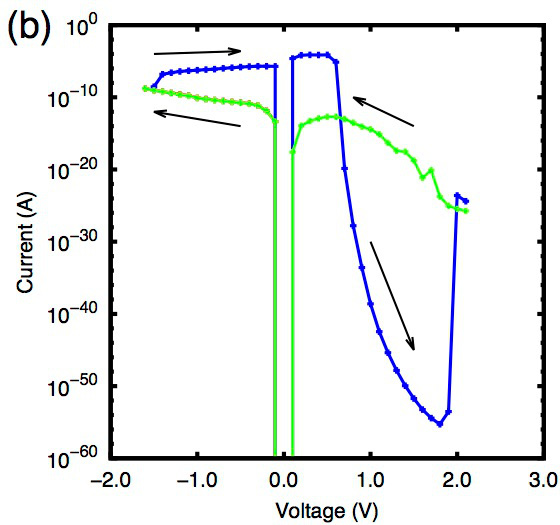
\includegraphics[height=4.5cm]{img/ixv-deff.jpg} 
      \caption{(a) sketch of the band bending inside the active layer of a memristor where the defect band is depicted as the dashed segment laying $E_d$ lower than CBM. (b) theoretical $i \times V$ curve obtained after changing the potential. The blue curve is the LRS while the green one is the HRS.} 
      \label{fig:ixvtheo-02} 
    \end{center}
  \end{figure}
\end{center}

In conclusion, the results presented in this chapter indicate that purely electronic mechanisms do play an important role in memristive switching. Using simple 1D models for both the electrostatic potential (solution to the Poisson equation) and the transmission probability (Schr\"odinger equation) we could derive multiple solutions to the memristor's potential barrier, show that these distinct solutions are stable and present a domain of coexistence of these solutions with respect to defect concentrations and device width. Consequently, the electronic current was obtained for to two simple mechanisms: tunneling and band-assisted tunneling. Even though the $i \times V$ curves do not capture all the features of the switching, it is evident that a qualitative agreement is achieved in comparison to experimental results. Still in the purely electronic mechanism picture, the consideration of other electronic transport models might lead to better agreement between the simulated and the experimental curves. Another approach would be the extension of the model to 2D or 3D, by solving both the Poisson equation and the Schr\"odinger equation in these dimensions, in a more realistic situation. The results presented here for the Poisson equation solver were submitted for publication, and the manuscript is attached in appendix \ref{sec:app-sub}.